\section{Value-Based and Policy-Based RL}
\begin{frame}{}
    \LARGE Reinforcement Learning: \textbf{Value-Based and Policy-Based Methods}
\end{frame}

\begin{frame}{Value-Based and Policy-Based RL}
\begin{columns}
\begin{column}{0.5\textwidth}
   \begin{itemize}
       \item \textbf{Value-Based Methods}
       \begin{itemize}
            \item Learn a value function
            \item Derive policy implicitly (e.g., $\varepsilon$-greedy)
       \end{itemize}
       \item \textbf{Policy-Based Methods}
       \begin{itemize}
            \item Do not learn a value function
            \item Learn the policy directly
       \end{itemize}
       \item \textbf{Actor-Critic Methods} \textit{(e.g.\ PPO, later today)}
       \begin{itemize}
            \item Learn both a value function and a policy
            \item Combines the strengths of both approaches above
       \end{itemize}
   \end{itemize}
\end{column}
\begin{column}{0.5\textwidth}
    \begin{figure}
    \centering
    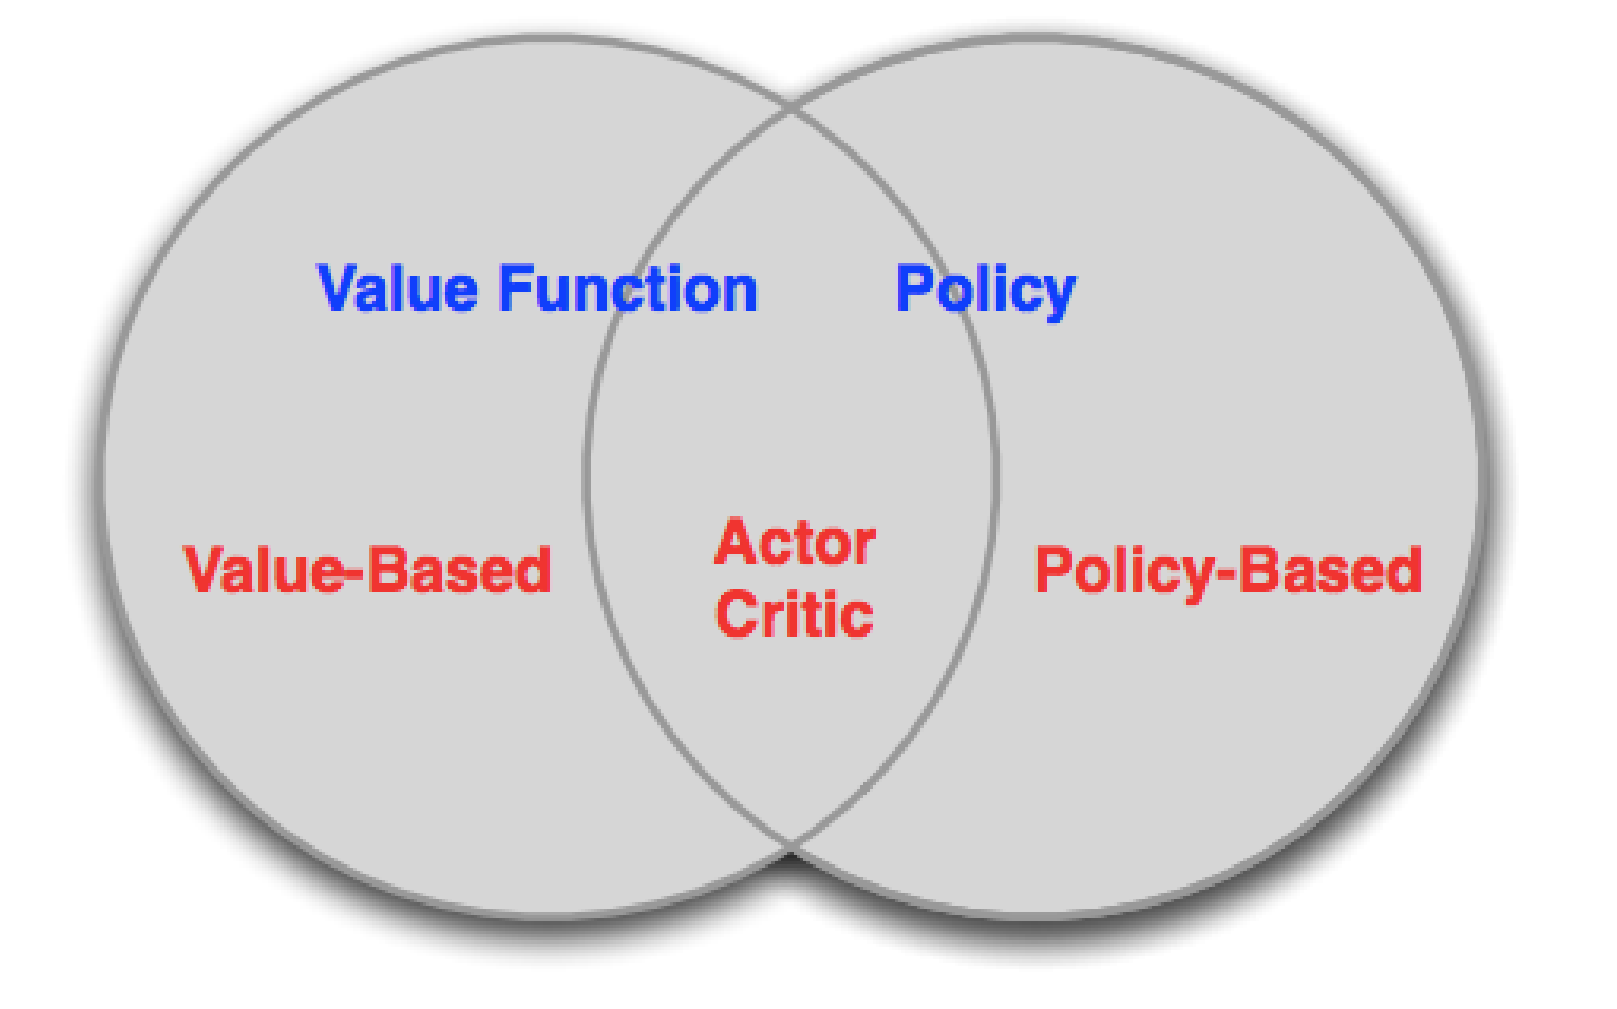
\includegraphics[width=1.0\textwidth,height=1.0\textheight,keepaspectratio]{images/vanilla-policy-gradient/a2c_2.png}
    \end{figure}
\end{column}
\end{columns}
\end{frame}


